% Copyright 2020  Ed Bueler

\documentclass[10pt,hyperref,dvipsnames]{beamer}

\mode<presentation>{
  \usetheme{Madrid}
  \usecolortheme{beaver}
  \setbeamercovered{transparent}  
  \setbeamerfont{frametitle}{size=\large}
}

\setbeamercolor*{block title}{bg=red!10}
\setbeamercolor*{block body}{bg=red!5}

\usepackage[english]{babel}
\usepackage[latin1]{inputenc}
\usepackage{times}
\usepackage[T1]{fontenc}
% Or whatever. Note that the encoding and the font should match. If T1
% does not look nice, try deleting the line with the fontenc.

\usepackage{empheq}
\usepackage{xspace,bm}
\usepackage{verbatim,fancyvrb}

\usepackage{tikz}
\usetikzlibrary{shapes,arrows.meta,decorations.markings,decorations.pathreplacing,fadings,positioning}

\usepackage{hyperref}

\newcommand{\ba}{\mathbf{a}}
\newcommand{\bb}{\mathbf{b}}
\newcommand{\bc}{\mathbf{c}}
\newcommand{\bbf}{\mathbf{f}}
\newcommand{\bg}{\mathbf{g}}
\newcommand{\bn}{\mathbf{n}}
\newcommand{\bq}{\mathbf{q}}
\newcommand{\br}{\mathbf{r}}
\newcommand{\bx}{\mathbf{x}}
\newcommand{\by}{\mathbf{y}}
\newcommand{\bv}{\mathbf{v}}
\newcommand{\bu}{\mathbf{u}}
\newcommand{\bw}{\mathbf{w}}

\newcommand{\bF}{\mathbf{F}}
\newcommand{\bG}{\mathbf{G}}
\newcommand{\bQ}{\mathbf{Q}}
\newcommand{\bU}{\mathbf{U}}

\newcommand{\bzero}{\bm{0}}

\newcommand{\grad}{\nabla}
\newcommand{\Div}{\nabla\cdot}
\newcommand{\minmod}{\operatorname{minmod}}

\newcommand{\CC}{\mathbb{C}}
\newcommand{\RR}{\mathbb{R}}

\newcommand{\ddt}[1]{\ensuremath{\frac{\partial #1}{\partial t}}}
\newcommand{\ddx}[1]{\ensuremath{\frac{\partial #1}{\partial x}}}
\newcommand{\Matlab}{\textsc{Matlab}\xspace}
\newcommand{\Octave}{\textsc{Octave}\xspace}
\newcommand{\eps}{\epsilon}

\newcommand{\ip}[2]{\left<#1,#2\right>}

\newcommand{\xiphalf}{{x_{i+\frac{1}{2}}}}
\newcommand{\ximhalf}{{x_{i-\frac{1}{2}}}}
\newcommand{\Fiphalf}{{F_{i+\frac{1}{2}}}}
\newcommand{\Fimhalf}{{F_{i-\frac{1}{2}}}}
\newcommand{\Fiphalfn}{{F^n_{i+\frac{1}{2}}}}
\newcommand{\Fimhalfn}{{F^n_{i-\frac{1}{2}}}}

\newcommand{\trefcolumn}[1]{\begin{bmatrix} \phantom{x} \\ #1 \\ \phantom{x} \end{bmatrix}}
\newcommand{\trefmatrixtwo}[2]{\left[\begin{array}{c|c|c} & & \\ #1 & \dots & #2 \\ & & \end{array}\right]}
\newcommand{\trefmatrixthree}[3]{\left[\begin{array}{c|c|c|c} & & & \\ #1 & #2 & \dots & #3 \\ & & & \end{array}\right]}
\newcommand{\trefmatrixgroups}[4]{\left[\begin{array}{c|c|c|c|c|c} & & & & & \\ #1 & \dots & #2 & #3 & \dots & #4 \\ & & & & & \end{array}\right]}

\newcommand{\blocktwo}[4]{\left[\begin{array}{c|c} #1 & #2 \\ \hline #3 & #4 \end{array}\right]}

\newcommand{\bqed}{{\color{blue}\qed}}
\newcommand{\ds}{\displaystyle}

\newcommand\mynum[1]{{\renewcommand{\insertenumlabel}{#1}%
      \usebeamertemplate{enumerate item} \,}}


\title{Glacier complementarity}
\subtitle{How to apply equations for where equations apply}

\author{Ed Bueler}

\institute[UAF]{University of Alaska Fairbanks}

\date{December 2020}

\AtBeginSection[]
{%
\begin{frame}
  \frametitle{Outline}
  \tableofcontents[currentsection,hideallsubsections]
\end{frame}
}

\begin{document}
\beamertemplatenavigationsymbolsempty

\begin{frame}
  \maketitle
\end{frame}

\begin{frame}
  \frametitle{Outline}
  \tableofcontents[hideallsubsections]
\end{frame}


\section{the views of two precise glaciologists}

\begin{frame}{W}

\begin{columns}
\begin{column}{0.5\textwidth}
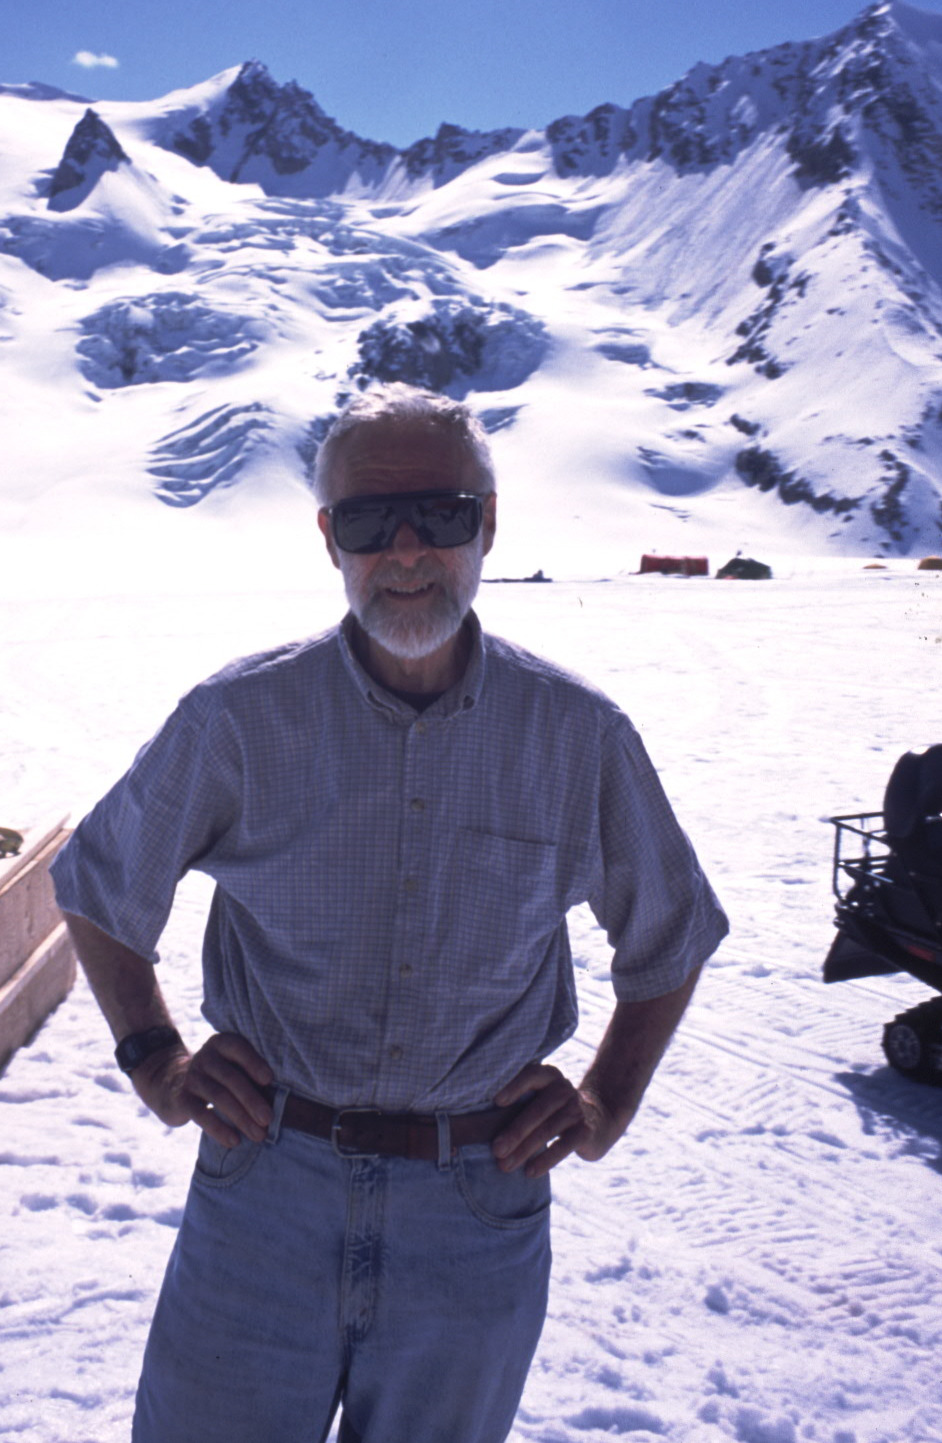
\includegraphics[width=0.8\textwidth]{figs/Will-by-Truffer.jpg}
%\url{https://news.uaf.edu/goodbye-to-a-raffish-glacier-scientist/}

\hfill \tiny \emph{photo by Martin Truffer} \phantom{dklfj asdlfj dslfaj}
\end{column}
\begin{column}{0.5\textwidth}
\begin{itemize}
\item W is a glaciologist
\invisible<1>{\item he is happy because he is standing on a glacier}
\invisible<1-2>{\item he can say two \emph{precise} things about his patch of the world}
\invisible<1-3>{\item one inequality and one equality}
\invisible<1-4>{\item<5>[$>$] the glacier thickness is positive
    $$H>0$$}

\vspace{-5mm}
\invisible<1-4>{\item<5>[$=$] the mass of ice is conserved
    $$\frac{\partial H}{\partial t} + \Div \left(\bU H\right) - a = 0$$}
\end{itemize}
\end{column}
\end{columns}
\end{frame}


\begin{frame}{A}

\begin{columns}
\begin{column}{0.5\textwidth}
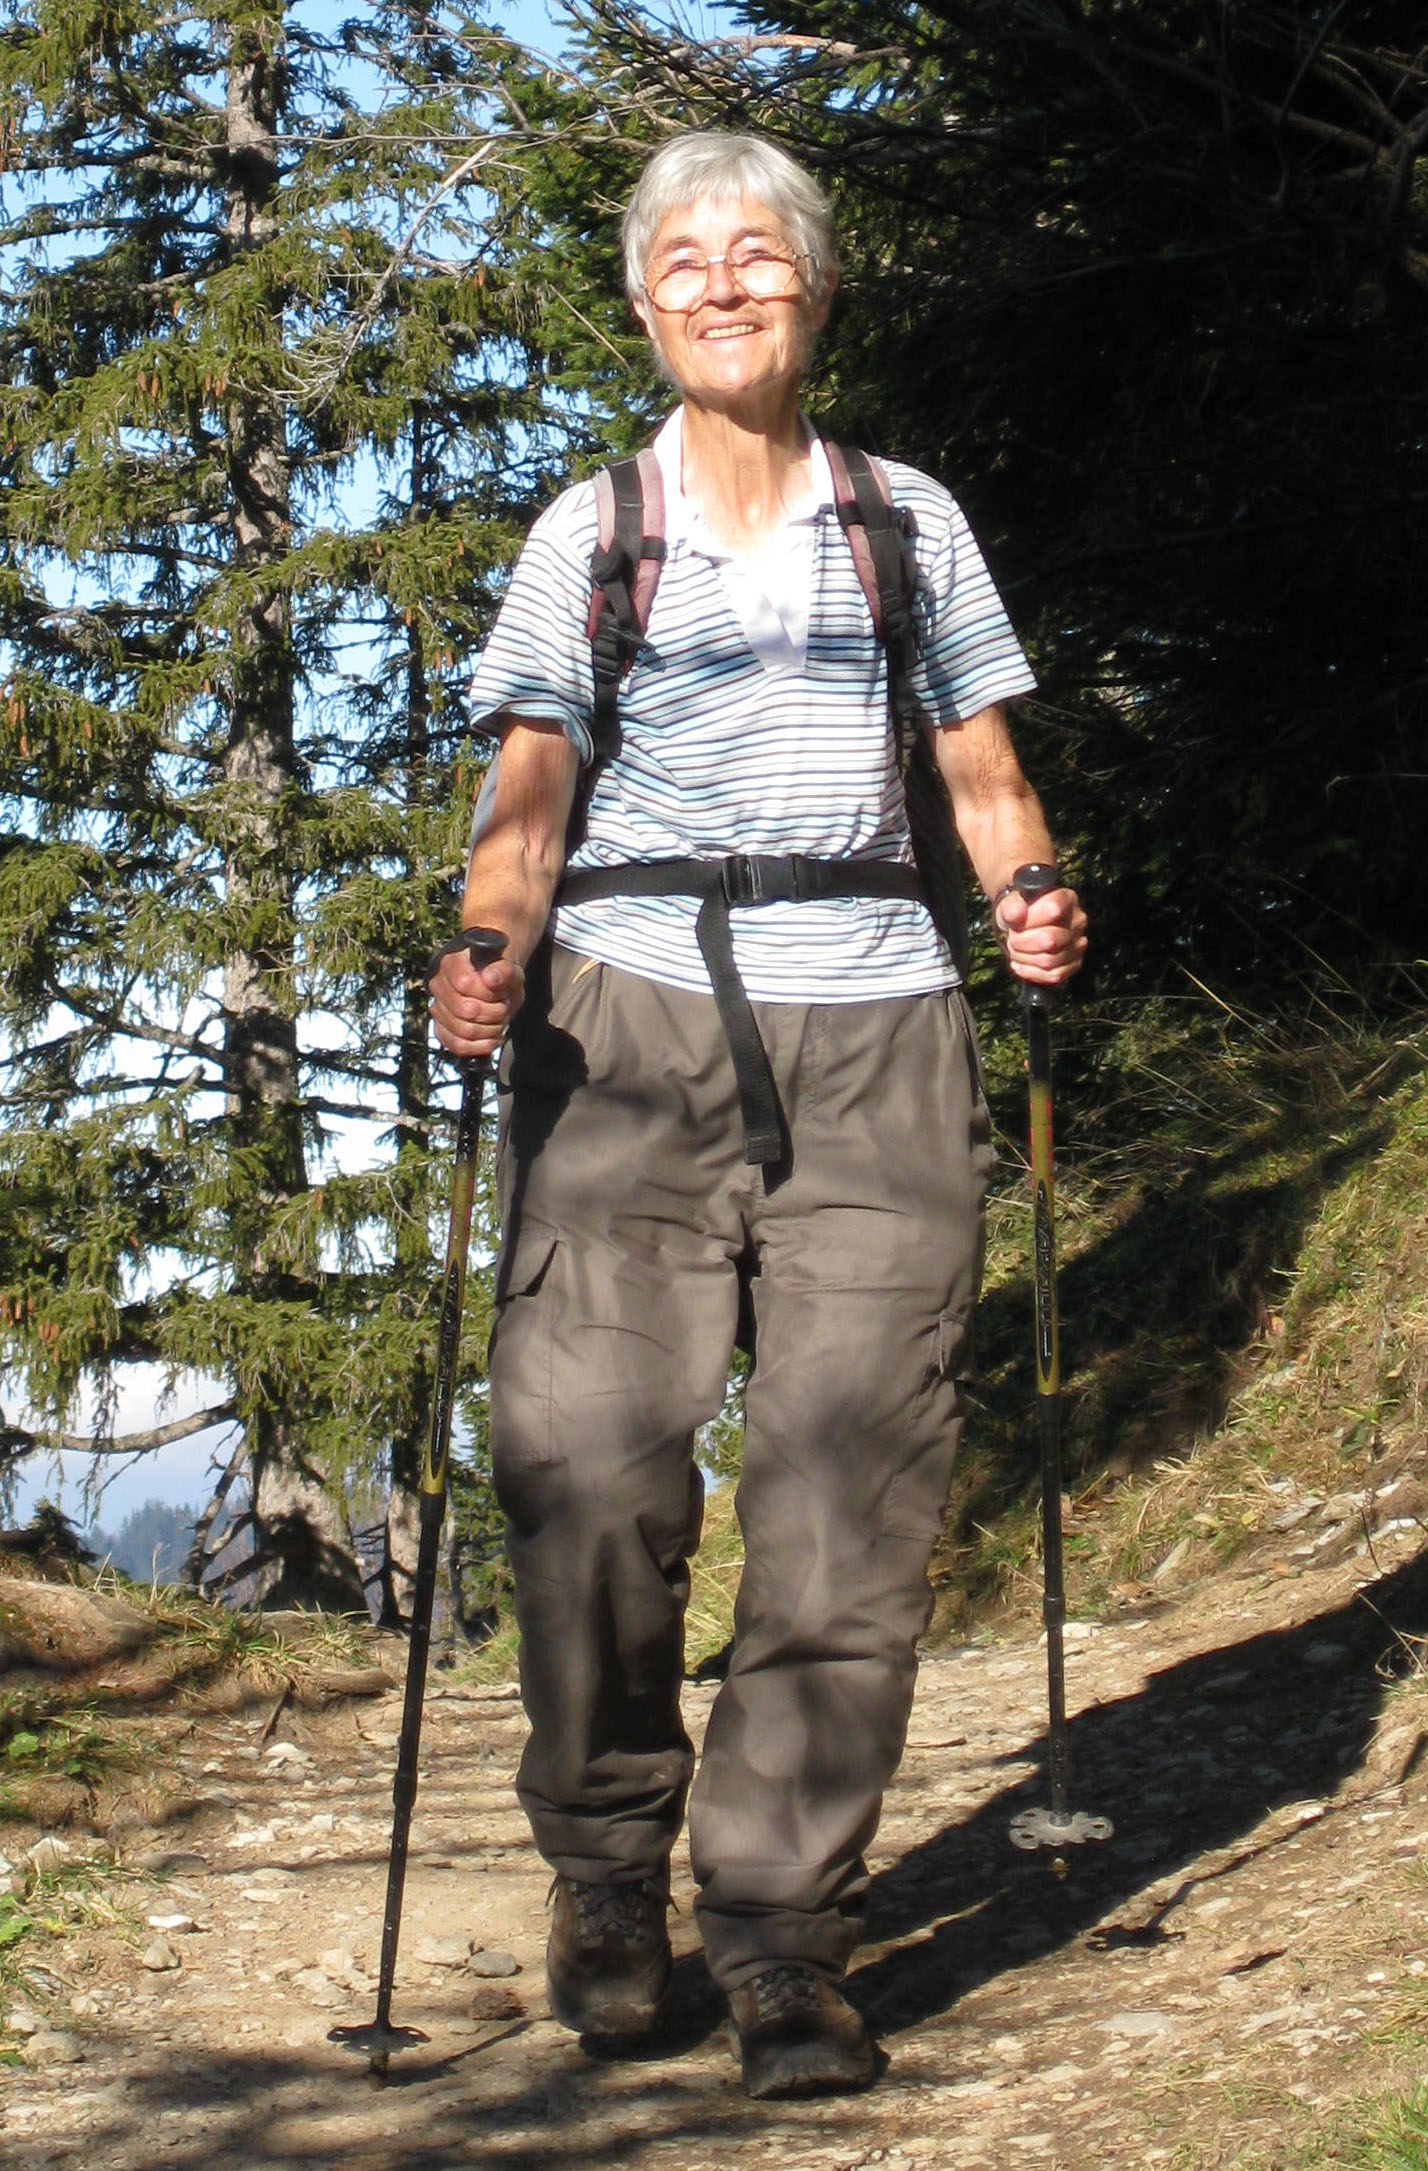
\includegraphics[width=0.8\textwidth]{figs/Iken_front_crop.jpg}
%\url{https://www.igsoc.org/awards/seligman/ikenseligman.html}
\end{column}
\begin{column}{0.5\textwidth}
\begin{itemize}
\item A is a glaciologist
\invisible<1>{\item she is not on a glacier, but happy to be hiking in the mountains}
\invisible<1-2>{\item she can say two \emph{precise} things about her patch of the world}
\invisible<1-3>{\item one equality and one inequality}
\invisible<1-4>{\item<5>[$=$] the glacier thickness is zero
    $$H=0$$}

\vspace{-5mm}
\invisible<1-4>{\item<5>[$>$] the annual surface mass balance is negative
    $$-a > 0$$}
\end{itemize}
\end{column}
\end{columns}
\end{frame}


\begin{frame}{two views in different patches}

\begin{columns}
\begin{column}{0.25\textwidth}
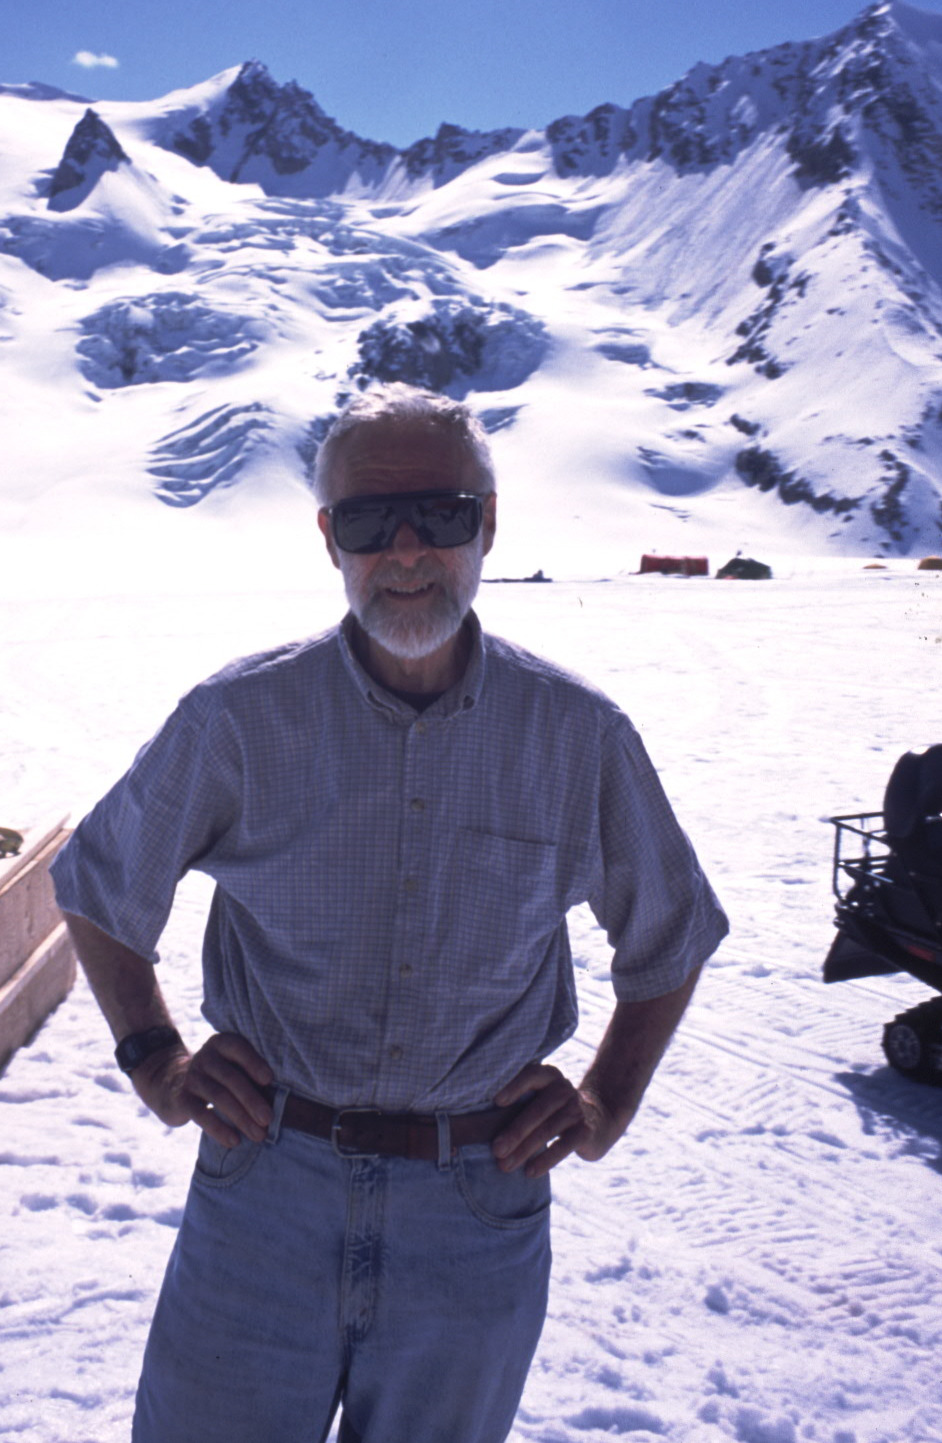
\includegraphics[width=0.7\textwidth]{figs/Will-by-Truffer.jpg}

\vspace{5mm}
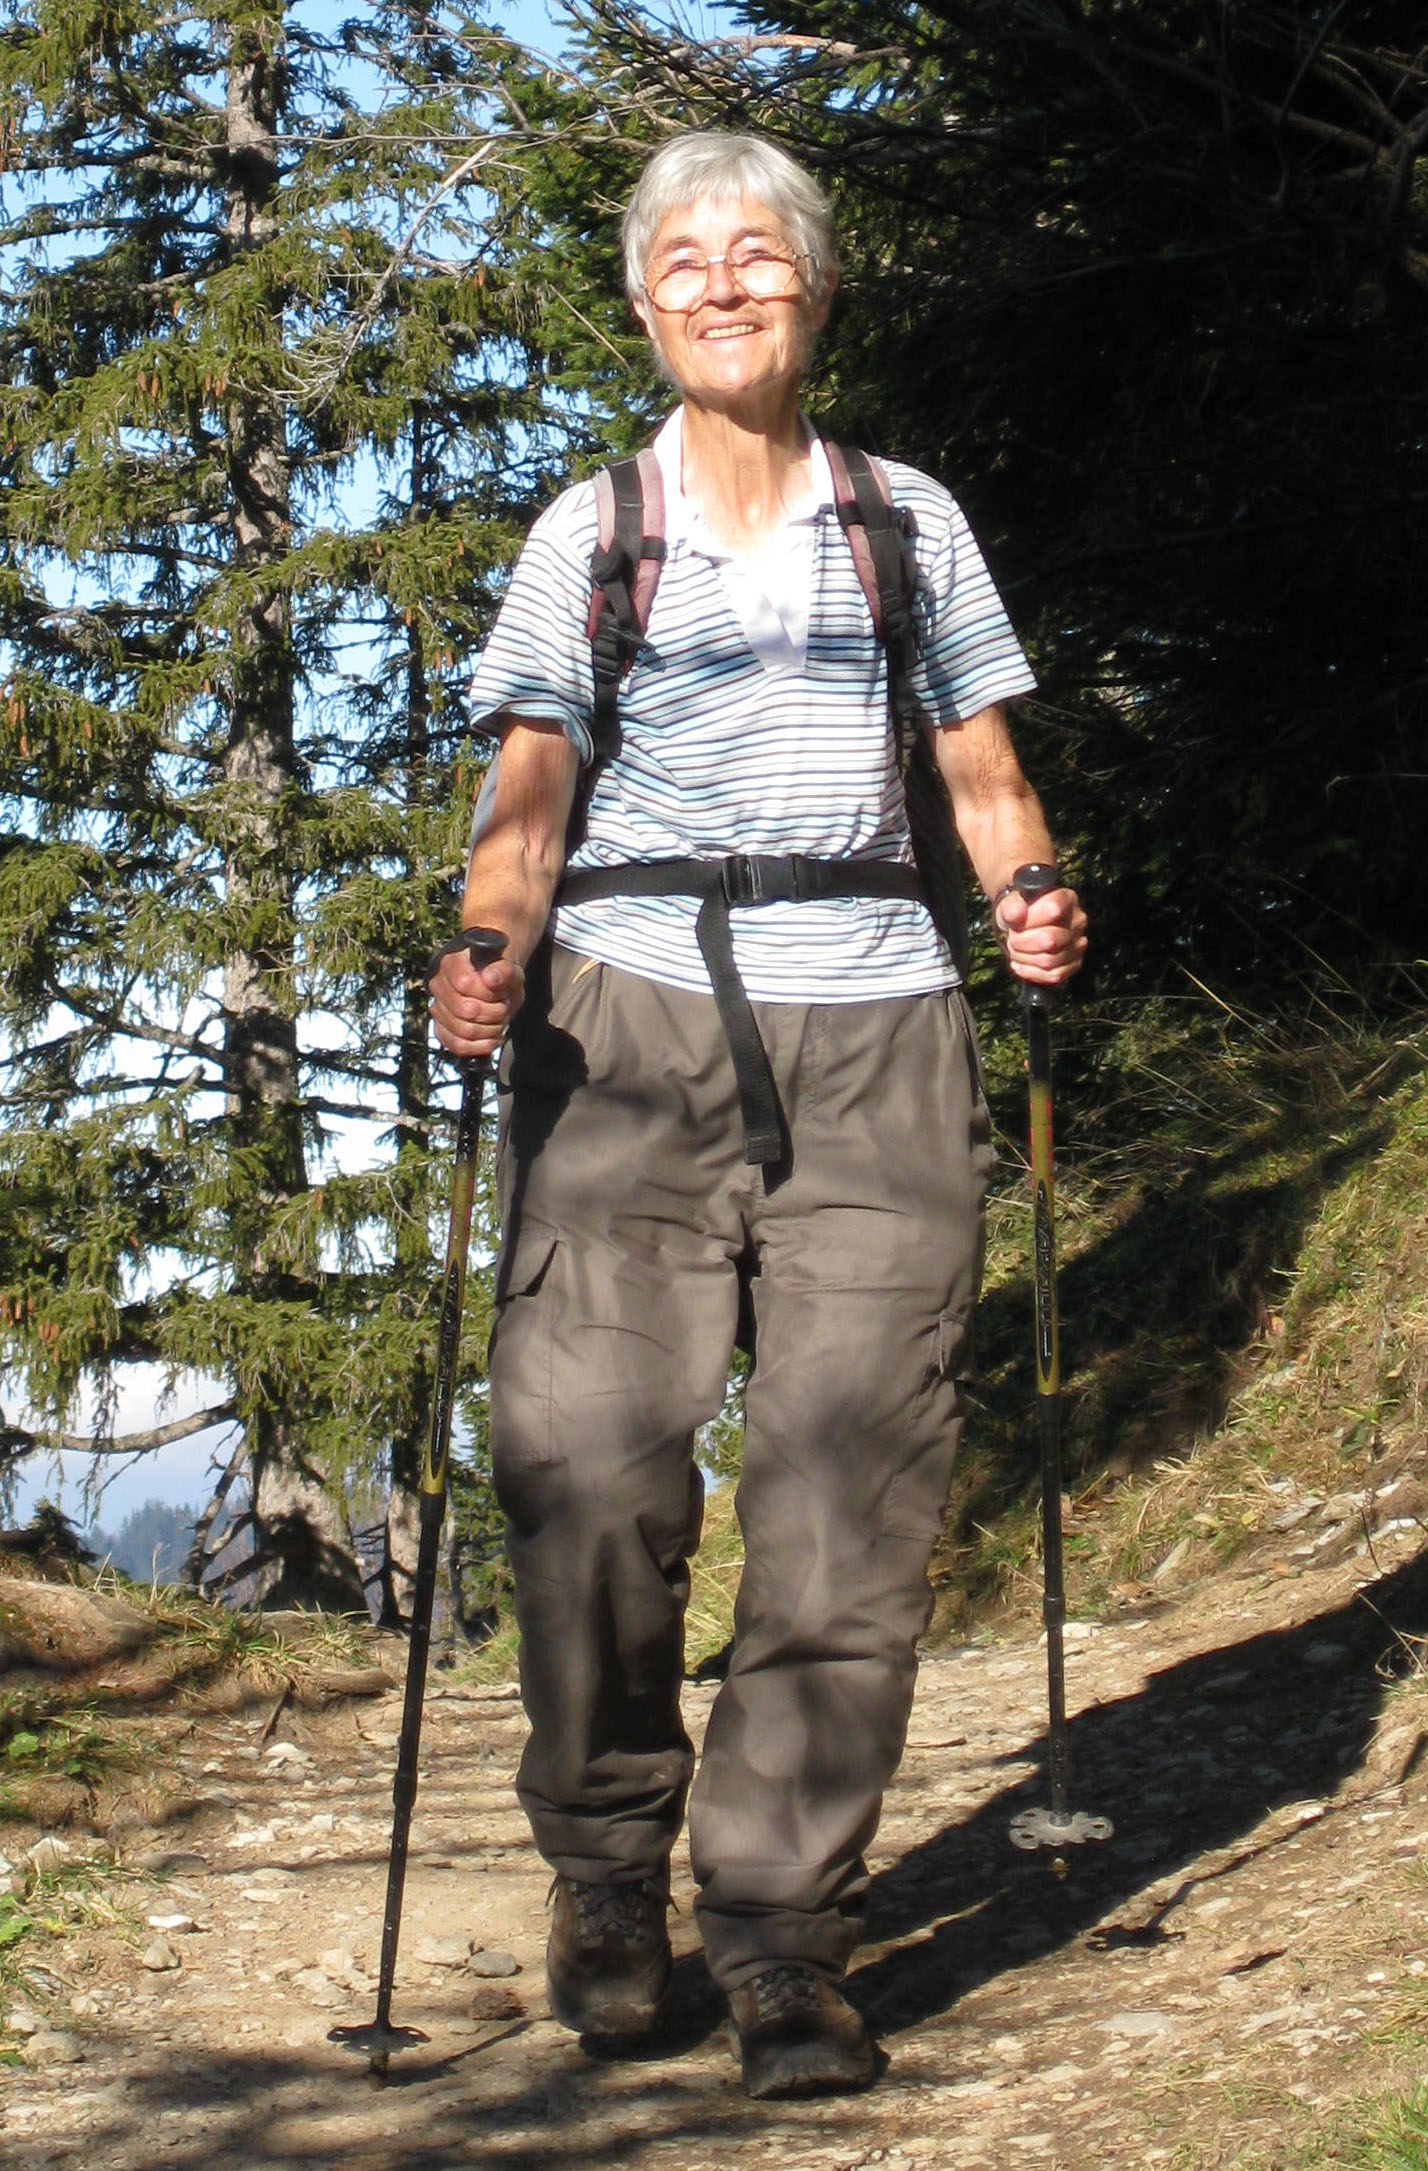
\includegraphics[width=0.7\textwidth]{figs/Iken_front_crop.jpg}

\bigskip

\bigskip
\end{column}
\begin{column}{0.75\textwidth}
\begin{itemize}
\item \emph{W says:} where I am
    \begin{itemize}
    \item[] the glacier thickness is positive
        $$H>0$$
    \item[] and mass of ice is conserved
        $$\frac{\partial H}{\partial t} + \Div \left(\bU H\right) - a = 0$$
    \end{itemize}
\item \emph{A says:} where I am
    \begin{itemize}
    \item[] the glacier thickness is zero
        $$H=0$$
    \item[] and the annual surface mass balance is negative
        $$-a > 0$$
    \end{itemize}

\medskip
\item<2> \emph{a skeptic says:} so what?  the world looks different in different places!
\end{itemize}
\end{column}
\end{columns}
\end{frame}


\begin{frame}{but first \dots define your terms}
\begin{itemize}
\item definitions.  \emph{please ask if you are unclear on some dumb symbol!}

\bigskip
\item $\bx = (x,y)$ is map-plane location
\item $t$ is time

\medskip
\item $H(t,\bx)$ is glacier thickness
\item $b(\bx)$ is bed elevation
\item $s(t,\bx)$ is glacier surface elevation
\item $a(t,\bx)$ is annual surface (climatic) mass balance
\item $\bU = \bU(t,\bx)$ is vertically-averaged horizontal ice velocity
\item $\bu = \bu(t,x,y,z)$ is ice velocity in 3D
\end{itemize}
\end{frame}


\begin{frame}{both views at once}
\begin{itemize}
\item both W's view and A's view arise from one set of equations:
\begin{align*}
H &\ge 0 \\
\frac{\partial H}{\partial t} + \Div \left(\bU H\right) - a &\ge 0 \\
H \left(\frac{\partial H}{\partial t} + \Div \left(\bU H\right) - a\right) &= 0
\end{align*}
\begin{itemize}
\item[$\circ$] ``equations'' in this talk usually means ``set of equations and inequalities''
\end{itemize}

\begin{itemize}
\item[$\circ$] \emph{consider}: W is standing on a glacier
\item[$\circ$] \emph{consider}: A is walking on a dirt trail
\end{itemize}

\invisible<1>{
\bigskip
\item<2> the third equation is \alert{complementarity}
\item<2> the whole thing is a \alert{(nonlinear) complementarity problem}
}
\end{itemize}
\end{frame}


\section{complementarity for glaciers}

\begin{frame}{what is true at a glacier margin?}

\begin{center}
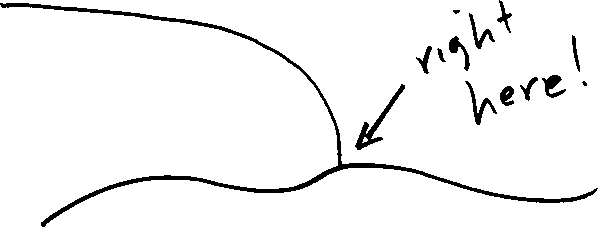
\includegraphics[width=0.4\textwidth]{figs/margin.png}
\end{center}

\begin{itemize}
\item the view switches at a glacier margin
\invisible<1>{
\only<1-2>{
\item<1-2> an extra equality holds at a margin:
   $$H=0 \qquad \text{\emph{and}} \qquad \frac{\partial H}{\partial t} + \Div \left(\bU H\right) - a = 0$$
}
\only<3>{
\item<3> \alert{an extra equality holds at a margin?}
   $$H=0 \qquad \text{\emph{and}} \qquad \frac{\partial H}{\partial t} + \Div \left(\bU H\right) - a \alert{\stackrel{?}{=}} 0$$
}
}
\end{itemize}
\end{frame}


\begin{frame}{useful to think about \emph{open sets}}

\begin{center}
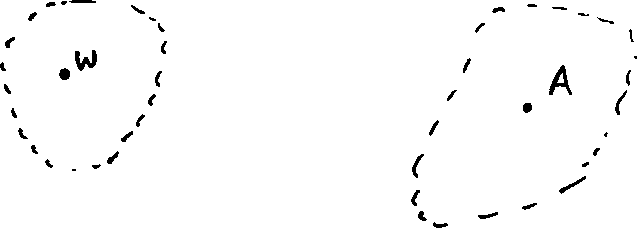
\includegraphics[width=0.4\textwidth]{figs/opensets.png}
\end{center}

\begin{itemize}
\item ``W is on a glacier'' means a neighborhood of glacier is around W
\item ``A is on a trail'' means a neighborhood of dirt is around A
\item ``neighborhood'' $=$ open set in the map-plane

\medskip
\item \emph{idea}:  a complementarity problem using derivatives, or any strong-form differential equation, only makes sense in open sets around locations

\medskip
\item a glacier margin has no neighborhood of differentiability of $H$ or $\bU$
\end{itemize}
\end{frame}


\begin{frame}{velocity or flux?}
\begin{itemize}
\item \dots and you might be worried about the zen question:

\begin{center}
\emph{what is the velocity $\bU$ of a glacier that isn't there?}
\end{center}

\vspace{5mm}
\item<2> let $\bq$ be the map-plane \emph{mass flux}
\item<2> it \emph{is} defined everywhere
\item<2> $\bq = \bU H$ \emph{on the glacier}
\item<2> mass conservation equation says \quad $\frac{\partial H}{\partial t} + \Div \bq = a$ \quad \emph{on the glacier}
\item<2> both $H$ and $\bq$ are zero outside the glacier
\item<2> dynamics determines flow from geometry, so: \quad $\bq=\bq(H)$
    \begin{itemize}
    \item[$\circ$] we can agree?: \quad $\bq(0)=\bzero$
    \end{itemize}
\end{itemize}
\end{frame}


\begin{frame}{what is \emph{actually} true at a glacier margin?}

\begin{center}
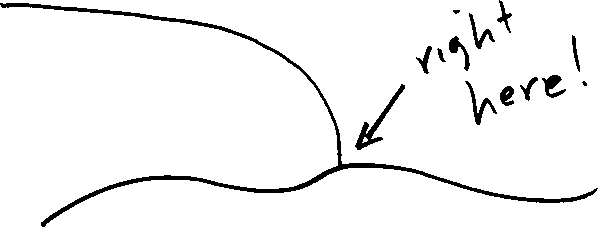
\includegraphics[width=0.4\textwidth]{figs/margin.png}
\end{center}

\begin{itemize}
\item \alert{both $H(t,\bx)$ and $\bq(t,\bx)$ are continuous in the map plane}
    \begin{itemize}
    \item[$\circ$] \dots in a fluids view of glaciers where thickness is well-defined
    \end{itemize}
\item so $H=0$ \emph{and} $\bq=\bzero$ at a glacier margin
    \begin{itemize}
    \item[$\circ$] true whether the margin is advancing, stationary, or retreating
    \end{itemize}
\item the quantity \quad $\frac{\partial H}{\partial t} + \Div \bq - a$ \quad jumps discontinuously
\end{itemize}
\end{frame}


\begin{frame}{applies everywhere, including where the glacier is}
\begin{itemize}
\item the complementarity problem applies \emph{everywhere on Earth}:
\begin{align*}
H &\ge 0 \\
\frac{\partial H}{\partial t} + \Div \bq - a &\ge 0 \\
H \left(\frac{\partial H}{\partial t} + \Div \bq - a\right) &= 0
\end{align*}
    \begin{itemize}
    \item[$\circ$] at the South Pole 1000 years ago
    \item[$\circ$] 1000 years from now in the middle of Death Valley
    \item[$\circ$] outside my door right now

    \medskip
    \item<2>[$\circ$] \emph{except} right at glacier margins
    \end{itemize}
\end{itemize}
\end{frame}


\begin{frame}{where is there glacier?}
\begin{itemize}
\item ``where is the glacier?'' is a first-class problem in glaciology
    \begin{itemize}
    \item[$\circ$] \emph{example}: determine ice sheet extent in past/future climates
    \end{itemize}
\item we want our theory and models to apply everywhere, so that we may answer this first-class problem \emph{within} a model
\item an NCP like
\begin{align*}
H &\ge 0 \\
\frac{\partial H}{\partial t} + \Div \bq - a &\ge 0 \\
H \left(\frac{\partial H}{\partial t} + \Div \bq - a\right) &= 0
\end{align*}
is the basis of such a model
    \begin{itemize}
    \item[$\circ$] the model also needs to compute $\bq$ given the geometry \dots it also needs to conserve momentum
    \end{itemize}
\end{itemize}
\end{frame}


\begin{frame}{my main point is that \dots}
\begin{itemize}
\item if you say ``my glacier model conserves mass'' then think
\begin{align*}
H &\ge 0 \\
\frac{\partial H}{\partial t} + \Div \bq - a &\ge 0 \\
H \left(\frac{\partial H}{\partial t} + \Div \bq - a\right) &= 0
\end{align*}
\emph{everywhere}, and not just
    $$\frac{\partial H}{\partial t} + \Div \bq = a$$
on the glacier

\medskip
\item<2> \dots and $H$, $\bq$, $a$ can be defined everywhere
\end{itemize}
\end{frame}


\begin{frame}{mass conservation or surface kinematical equation?}
\begin{itemize}
\item FIXME SKE 
\item applies even without incompressibility
\item not really a more-fundamental view because I am assuming $s \leftrightarrow H$ are well-defined, a restriction on glacier geometry
\end{itemize}
\end{frame}


\begin{frame}{xx}
\begin{itemize}
\item xx
\end{itemize}
\end{frame}


\section{complementarity from optimization}

\begin{frame}{abstract inequality-constrained optimization}
\begin{itemize}
\item xx
\end{itemize}
\end{frame}

\begin{frame}{example: obstacle problem}
\begin{itemize}
\item xx
\end{itemize}
\end{frame}

\begin{frame}{equivalences}
\begin{itemize}
\item e.g. obstacle problem:

(constrained optimization) $\leftrightarrow$ (variational inequality) $\leftrightarrow$ (NCP)
\item ice:

\phantom{(constrained optimization) $\leftrightarrow$} (variational inequality) $\leftrightarrow$ (NCP)
\end{itemize}
\end{frame}


\section{consequences for modelers (\emph{and real scientists too})}

\begin{frame}{it runs}
\begin{itemize}
\item FIXME works with NCP solver and Newton method as in SIAFVE: provide $a$ and $b$ on $\Omega$, give initial guess for $s$, and say ``go''
\item FIXME current project: make it Stokes
\item for implicit time steps
\end{itemize}
\end{frame}

\begin{frame}{discrete mass conservation}
\begin{itemize}
\item FIXME at the free boundary is impossible; see layer paper
\item bounds on mass accounting errors
\end{itemize}
\end{frame}

\begin{frame}{A's view is more interesting}
\begin{itemize}
\item \emph{A says:} even when one is just walking down a trail, precise glaciology is possible
\item FIXME glossary could define surface mass balance $a$ as the ``official'' quantity that makes the $(H,F(H))$ NCP true
\end{itemize}
\end{frame}

\begin{frame}{surface mass balance should be modeled (almost) everywhere}
\begin{itemize}
\item FIXME for implicit time steps, its essential
\item FIXME thought experiment: need ice-surface case [piston of ice cartoon], need snow-surface case [ditto]
\end{itemize}
\end{frame}


\begin{frame}{are there big ideas in glaciology?}
\begin{itemize}
\item I am not sure most glaciologists have an opinion on this
\item I disagree

\bigskip
\item<2> some ``big ideas'':
    \begin{itemize}
    \item[$\circ$] volume-area scaling \quad \emph{$\longleftarrow$ Will worked on this!}
    \item[$\circ$] ``glaciology is a 1 bar subject''
    \item[$\circ$] hysteresis of glacier volume from elevation dependence of mass balance
    \item[$\circ$] the tidewater glacier cycle
    \item[$\circ$] mass/energy/momentum conservation \quad ?
    \item[$\circ$] complementarity gives extent and margins \quad ?
    \end{itemize}
\end{itemize}
\end{frame}


\begin{frame}{remembering}

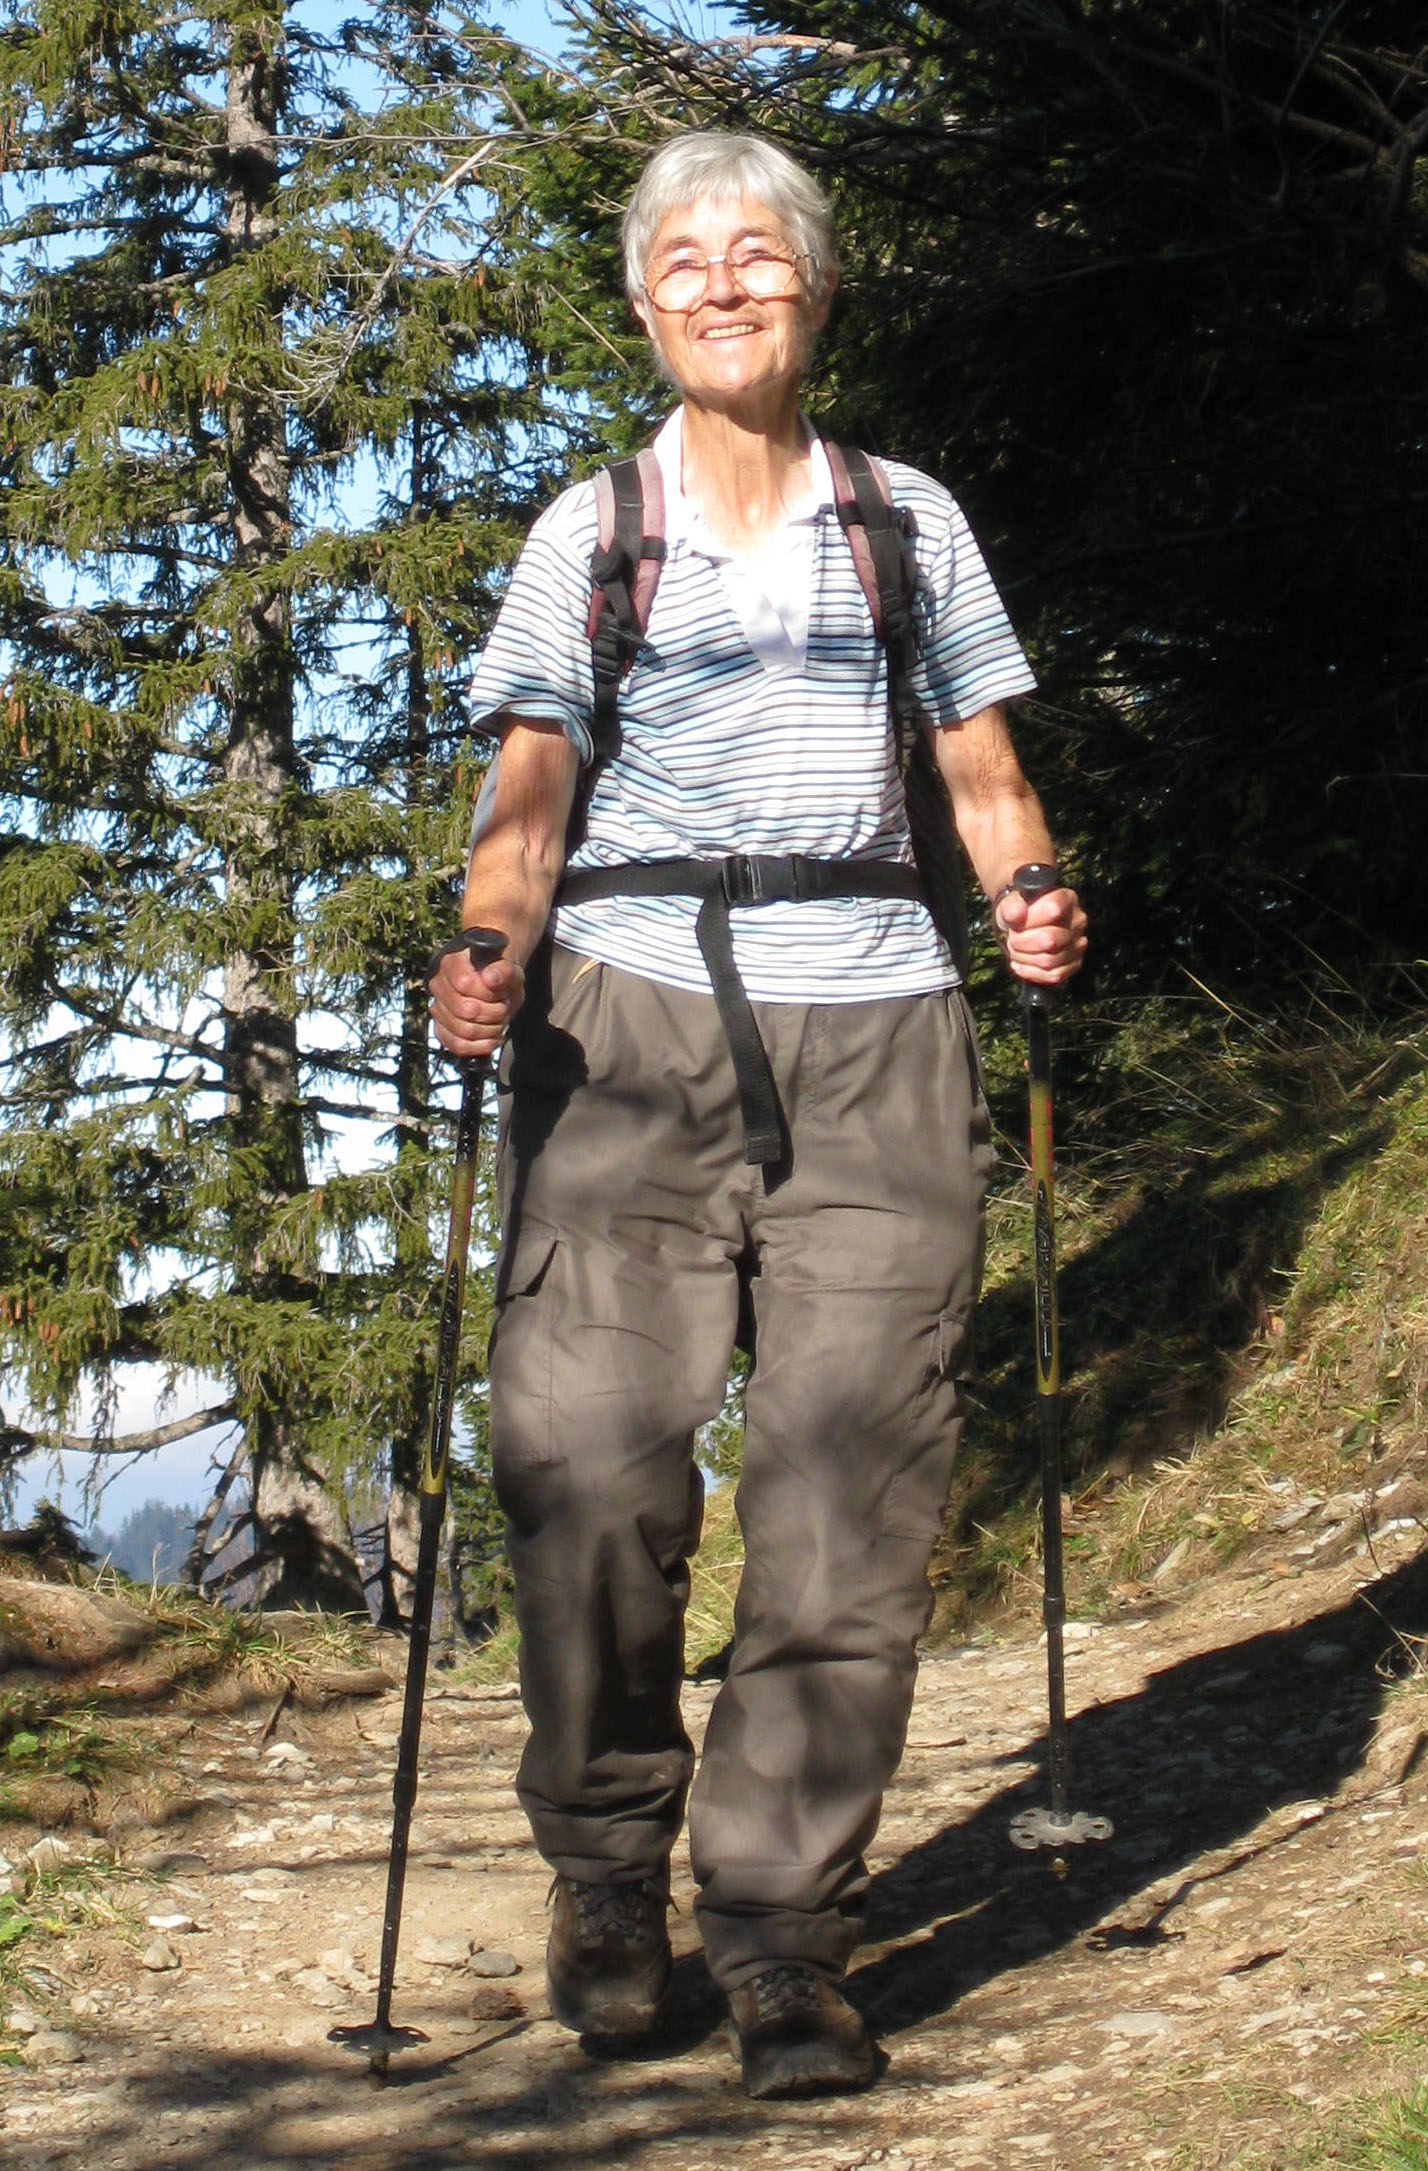
\includegraphics[width=0.4\textwidth]{figs/Iken_front_crop.jpg} \hfill 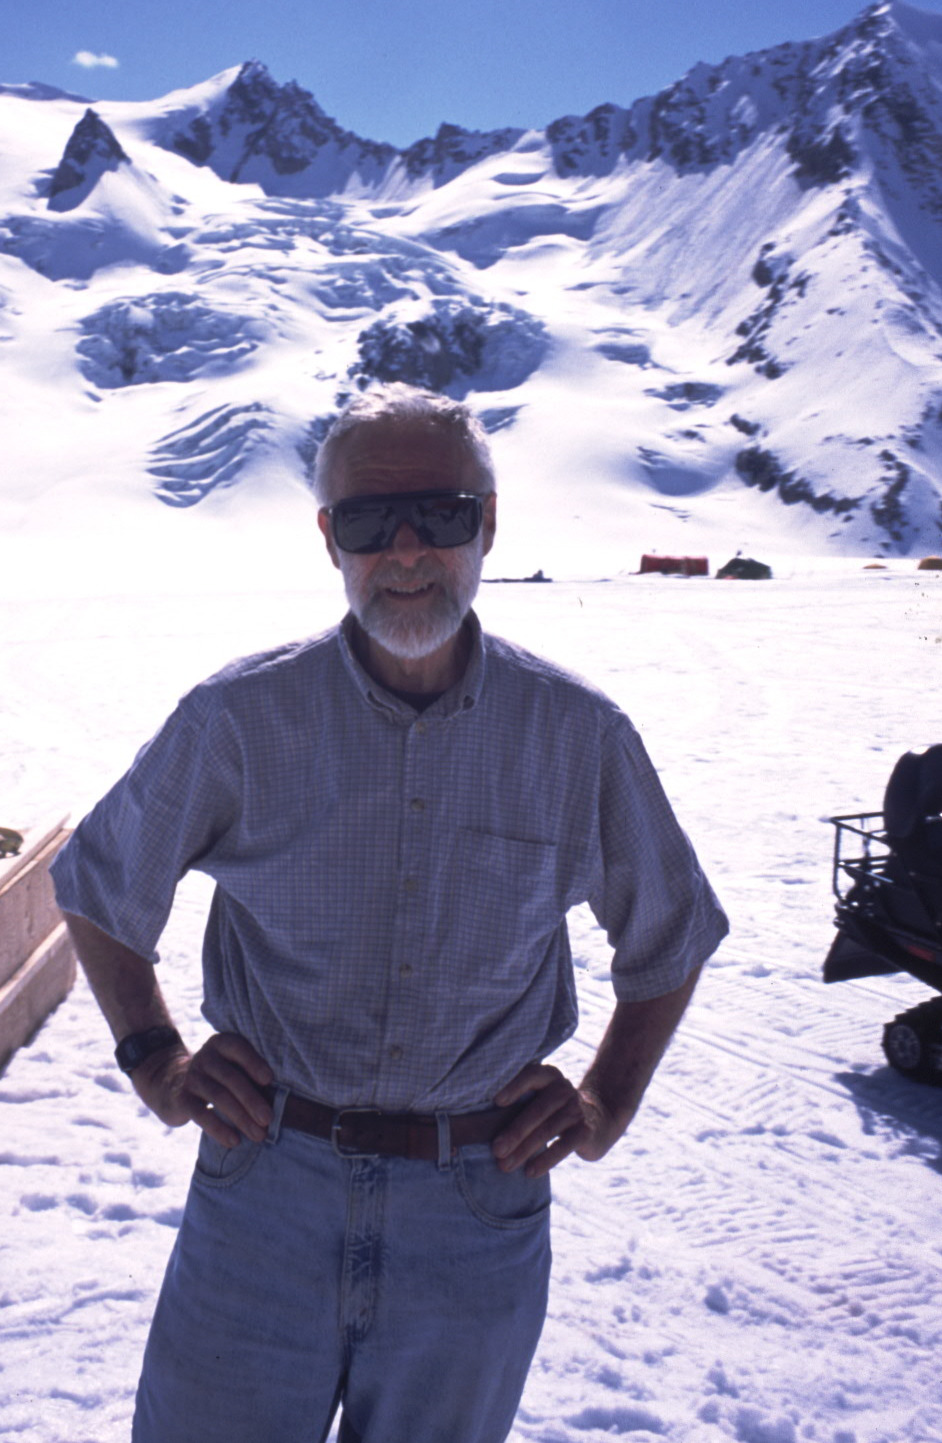
\includegraphics[width=0.4\textwidth]{figs/Will-by-Truffer.jpg}

Almut Iken (1933--2018) \hfill Will Harrison (1936--2020)
\end{frame}


\end{document}

